\section{Back projection and filtered back projection}
One can now ask if it is possible to go back from a sinogram to an image, and in fact it is. Two common image reconstruction techniques which can be applied if a sinogram is obtained is back projection and filtered back projection. With back projection the response measured from the obtained projections are uniformly distributed back along the lines the line integrals were computed. Doing this for several projections results in areas where the reconstructed image will get more exposure, and thus a rough / blurred outline will appear. This is sketched in \autoref{backprojection} where we see object A and B would emerge in the reconstruction because the obtained responses from the projections will intersect at these locations. A back projection can be seen in \autoref{reconbackprojection}.\\
\begin{figure}
	\centering
	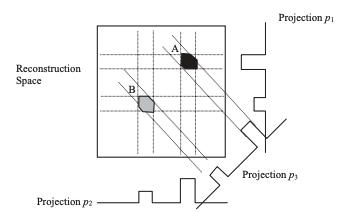
\includegraphics[width=0.9\linewidth]{Materials/backprojection}
	\caption{Illustration of back projection. By uniformly distribute the response from the obtained projections back along the line it was obtained a blurred reconstruction can be obtained. Image taken from \cite{MIA}.}
	\label{backprojection}
\end{figure}
\begin{figure}
	\centering
	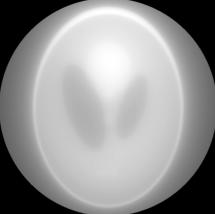
\includegraphics[width=0.6\linewidth]{Materials/reconnofilter}
	\caption{Result of a back projection made with the library \textit{skimage} setting the \textit{filter} parameter of the \textit{iradon} function to 'None'.}
	\label{reconbackprojection}
\end{figure}
To achieve sharper results, the filtered back projection is used. In filtered back projection the obtained projections are taken into frequency space by computing the 1D Fourier transform. The Fourier Slice Theorem then establishes a relationship between $F(u,v) = \mathcal{F}\{f(x,y)\}$ and $P(\mathcal{E},\theta) = \mathcal{F}\{p_{\theta}(p)\}$ where $P(\mathcal{E},\theta)$ is equivalent to the part of $F(u,v)$ that falls on a radial line with angle $\theta$. That is, by computing the Fourier transform of the 1D projections and using the Fourier Slice Theorem, we obtain a single line in 2D frequency space. By adding several projections together in this way we end with a 'filled' frequency space and we can then take the 2D inverse Fourier transform and get an approximation to the original function $f(x,y)$. In \autoref{filteredbackprojection} an outline of this process is sketched.\\
\begin{figure}
	\centering
	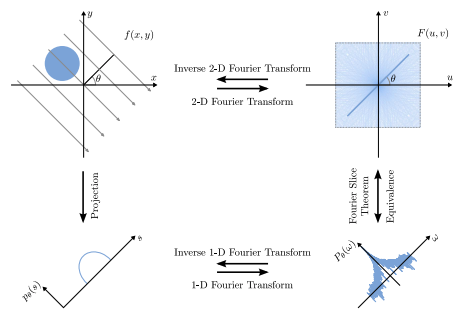
\includegraphics[width=\linewidth]{Materials/filteredbackprojection}
	\caption{Illustration of filtered back projection. First a projection is made, the its Fourier transform is computed. The Fourier Slice Theorem is then used to bring the 1D signal into a 2D line. Several lines can then be added together to 'fill' the frequency space. Finally an inverse Fourier transform can then be used to approximate the original function. Image taken from \cite{MIS}.}
	\label{filteredbackprojection}
\end{figure}
A slight issue to simply implement this pipeline is, the further out towards the endpoints of the lines in the frequency space we go, i.e. the more frequencies we include, the further the distance becomes between the lines, and thus the less information we have. To get more information one could simply sample more lines, i.e. obtain more projections, however, this would both be time consuming and expose the patient for more radioactivity. Instead one can limit the frequencies used by simply doing a cutoff at a certain 'max frequency'. However, as all the lines always will go through the origin, the lower frequencies are likely to be over represented. A Ram-Lak filter, shown in \autoref{ramlak}, is thus often used. This filter suppresses low frequencies while amplifying high, under sampled, frequencies, while providing a cutoff at some max frequency. Using the filter is also cheap in terms of efficiency as we are already in frequency space where a multiplication with the Ram-Lak filter will result in a convolution with it in the spacial domain.\\
\begin{figure}
	\centering
	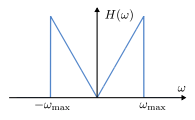
\includegraphics[width=0.7\linewidth]{Materials/RamLak}
	\caption{The Ram-Lak filter. Image taken from \cite{MIS}.}
	\label{ramlak}
\end{figure}
A common use case for filtered back projection is CT reconstruction, where after the CT scan one gets a number of projections which then can be used to approximate the original object scanned. 